\documentclass[oneside, a4, titlepage]{scrartcl}

\usepackage{graphicx}
\usepackage[american]{babel}
\usepackage{umlaute}
\usepackage{picture}
\usepackage{tabularx}
\usepackage{trfsigns}
\usepackage{prettyref}
\usepackage{titleref}
\usepackage{nameref}
\usepackage{subfig}
\usepackage{bm}
\usepackage{adjustbox}
\usepackage{varwidth}
\usepackage{amsmath,amssymb}
\usepackage{amsthm}
\usepackage{tikz-uml}
\usepackage[underline=false]{pgf-umlsd}
\usepackage[colorlinks, pdfpagelabels, pdfstartview = FitH, bookmarksopen = true, bookmarksnumbered = true,
linkcolor = black, plainpages = false, hypertexnames = false, citecolor = black, pagebackref = true, pdftex, pdfauthor={Berkay K�ksal, Alexander K�chler, Saad Lamdouar}, pdftitle={Ready2Meet: Event Organizer}] {hyperref}

\titlehead{\centering
\includegraphics[width=6cm]{graphics/EurecomLogo.png}}
\title{MobServ Challenge Project 2017}
\subtitle{Ready2Meet: Event Organizer for Android}
\author{Berkay K\"oksal \and Alexander K\"uchler \and Saad Lamdouar}
\date{\today}
\publishers{\centering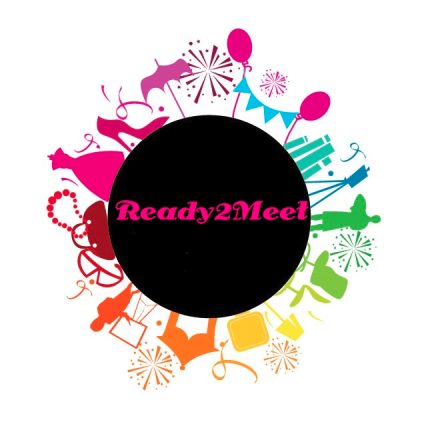
\includegraphics[width=6cm]{graphics/Ready2Meet_Logo.png}} % We have no publishers but a logo we want to show ;)

\renewcommand{\arraystretch}{1.25}
\newcolumntype{C}{>{\centering\arraybackslash}X}

% Stuff for UML Sequence
\renewcommand{\mess}[4][0]{
  \stepcounter{seqlevel}
  \path
  (#2)+(0,-\theseqlevel*\unitfactor-0.7*\unitfactor) node (mess from) {};
  \addtocounter{seqlevel}{#1}
  \path
  (#4)+(0,-\theseqlevel*\unitfactor-0.7*\unitfactor) node (mess to) {};
  \draw[->,>=angle 60] (mess from) -- (mess to) node[midway, above]
  {#3};    
}

\usepackage{enumitem}
\setlist{itemsep=0.1em}

\begin{document}
\maketitle

%\setcounter{tocdepth}{2}
%\tableofcontents
%\newpage

\section{Application Description}
The event organizer (name: Ready2Meet) is an Android app to facilitate creating events and inviting people. The core of the application, namely organizing an event, can be used in two different modes:
\begin{enumerate}
\item Planned event
\item Spontaneous event
\end{enumerate}

For both modes, the user creates an event (including a start and end time, location, type of event and eventually a name). In the planned event mode, the user can invite specific people (friends) while for the spontaneous event, it is also possible to send an invitation to people which are close to the user's current location. Like this, he is able to spontaneously gather people based on their location.

Apart from this, all people joining an event should be able to share pictures of the event in the app and influence the event's outcome e.g. by voting for music on a party. Also, a chatroom should be available to communicate with the people before or after the event.

For all kinds of events, the organizing person can add a list of required material (e.g. drinks or food) so that the guests can register to bring some of the material and thus easing the organization.

Finally, every user invited to an event is provided additional information like the weather forecast for outdoor events and whether he is available on the date when the event is scheduled.

\section{Features}
The features of our event organization app include
\begin{itemize}
\item Create an event (e.g. party, sports, hiking, lunch, ...)
	\begin{itemize}
	\item Invite friends
	\item Invite people in a close area. I.e., the user can specify a radius to invite people and the people are notified if they are interested in this kind of events
	\end{itemize}
\item Chatroom for event
\item Enable music organization/voting during the event
\item Share pictures of the event
\item Who brings what?
\item Get some additional information for the event 
	\begin{itemize}
	\item Weather forecast for outdoor events
	\item Check if timeslot is free in your calendar
	\end{itemize}
\item Share the event in other networks e.g. on facebook
\end{itemize}

We therefore plan to use Google API (maps), firebase database to provide a real time database, and OpenWeatherMap API to retrieve the weather forecast.

\section{Developer Team}
The team consists of three people:
\begin{itemize}
\item Saad Lamdouar: UI developer
\item Berkay K\"oksal: Core developer
\item Alexander K\"uchler: Core developer
\end{itemize}

\section{Business Model}
Different business models are possible to push the app on the market. In this section, we discuss potential models and pricing strategies and finally chose the most promising model. Furthermore, we discuss a marketing strategy for our application.

\subsection{Monetization}
A completely free (e.g. open source) app is the first possibility. While this potentially targets the highest number of users as the app is free to use and accessible also in alternative stores like F-Droid, the application would not lead to any profit.

A second option is to use advertisements in the app in order to gain from the application. While this leads to a higher income, it contradicts the open-source strategy and thus would probably lead to a smaller target group. However, as the vast majority of Android users install apps from the Google Play Store, the decrease of users is acceptable.

Together with the app using advertisement, it is possible to offer an for a small price and without ads. An app which has only a priced version does not appear to be promising to us as most users will not be willing to pay for the service.

Also, In-App sales would be possible e.g. to enhance the possibilities of a user when creating events.
In especial, this makes sense for business customers that could use the application to advertise their business. A possible scenario is creating events in the application which reflects the companies product portfolio (e.g. guided tours, sports, parties in a bar, \dots). Like this, the company can acquire new customers which are nearby e.g. during their holidays and thus our app presents a new marketing strategy. In the scenario of commercial users, it would be possible to earn a reward for every user which joins the respective event due to our platform. The reward could be negotiated as a percentage of the tickets for the event or as a fixed amount. However, both cases would require to include a ticket-selling system for the billing. This would be a possible extension of the app.

In our case, the most promising strategy is to offer a free app with advertisements as well as a paid version without ads. In-App sales which target commercial customers of the app can make the app more powerful. E.g. an event could be permanent or the radius to invite people could be extended. Also, the creators of an event could have additional possibilities.

\subsection{Marketing Strategy}
As our app aims at making events available to the highest possible number of potential participants, organizing events is the main possibility to advertise the app.

First, it is possible to offer free events to users which are organized by us. Second, we could offer discounts to our users for paid events which are organized by a third party. This is beneficial for both, the organizing party as they get additional participants and us, as we can make our app attractive for many users and thus gain a high number of users.

Both techniques aim at attracting as many users as possible. Even if we have some expenses for the events and eventually for offering the discounts, this can decline once we have sufficient customers.

\subsection{Competitors}
In this section, we shortly present a couple of competitors. Please note that the list is not complete and only presents a rough overview of the market.

Fever generates an event list taking into account the user's interests. However, it is only available in a few big cities and does not offer many events. Also, the focus is on commercial events while we aim at providing a platform to offer any kind of events, in especial, ``private'' and free ones.

WeTorch is a free app that provides a selection of events which are close to the user's location. It only exists in spanish and the focus lies on cultural events as well as arts.

Event Manager and Event Manager by Billeto give overviews of the event for event managers and help event organizers to grow their event reach and manage it.

While offering a platform is not the main focus, Facebook provides the functionality to invite friends to events or make them publicly available. In especial due to the large user community, it is an important competitor on the market.

\section{Implementation}
In this section, we discuss technical details of our implementation.

\subsection{Database}
To store our data (events, messages, users) and make them available to all users, we heavily make use of the features of Firebase\footnote{\url{https://firebase.google.com/}} database. Firebase provides a real-time database and is therefore ideally suitable to make changes on data available to multiple users in real time. Apart from that, it can easily be integrated into Android apps (as well as iOS and web applications).

We need to store 3 different types of data structures namely user accounts, chat messages and events. For each of the structures, one java class defines the data fields which are stored. Class diagrams of the classes are shown in \autoref{fig:dbClasses}.

\begin{figure}[htb]
\centering
\begin{tikzpicture}[every node/.style={scale=0.8}]
\umlclass{fr.eurecom.Ready2Meet.database::User}{
+ DisplayName : String\\
+ ParticipatingEvents: Map\textless String, Boolean\textgreater\\
+ ProfilePictureURL : String
}{} (User);

\umlclass[below of=User, node distance=3.5cm]{fr.eurecom.Ready2Meet.database::Message}{
+ message : String\\
+ senderId : String\\
+ time : String
}{} (Message);

\umlclass[below of=Message, node distance=10cm]{fr.eurecom.Ready2Meet.database::Event}{
+ id : String\\
+ title : String\\
+ description : String\\
+ owner : String\\
+ current : Long\\
+ categories : Map\textless String, Boolean\textgreater\\
+ capacity : Long\\
+ picture : String\\
+ place : String\\
+ startTime : String\\
+ endTime : String\\
+ Participants : Map\textless String, Boolean\textgreater\\
%+ WhoReported Map\textless String, Boolean\textgreater\\
+ notificationArea : Long\\
+ latitude : Double\\
+ longitude : Double
}{};
\end{tikzpicture}
\caption{UML class diagrams of the database classes}
\label{fig:dbClasses}
\end{figure}

\subsection{Application Components}
To provide the functionality, we implemented several different components which we discuss in this section.

The first crucial components of any Android app are the Activities shown in \autoref{fig:activities}. First, the three activities \texttt{ResetPasswordActivity}, \texttt{SignupActivity}, \texttt{LoginActivity} are responsible for managing user accounts and the corresponding login credentials. The class \texttt{ChatActivity} shows the chatroom for a selected event and requires the ID of the event in an extra in order to retrieve the chat messages. \texttt{AddEventActivity} is used to add one new event to the event database. The \texttt{MainActivity} shows the start screen of the app and displays all events on a map as well as in a list.

\begin{figure}[htb]
\centering
\begin{tikzpicture}[every node/.style={scale=0.8}]
\umlsimpleclass{AppCompatActivity}
\umlsimpleclass[type=interface, x=8]{OnNavigationItemSelectedListener}
\umlsimpleclass[type=abstract, x=11.3, y=-2]{ToolbarActivity}
\umlsimpleclass[x=-2, y=-2]{ResetPasswordActivity}
\umlsimpleclass[x=2, y=-2]{SignupActivity}
\umlsimpleclass[x=5.3, y=-2]{LoginActivity}
\umlsimpleclass[x=8.3, y=-2]{ChatActivity}
\umlsimpleclass[x=11.3, y=-4]{MainActivity}
\umlsimpleclass[x=8, y=-4]{AddEventActivity}

\umlimpl{ToolbarActivity}{OnNavigationItemSelectedListener}
\umlVHVinherit{ToolbarActivity}{AppCompatActivity}
\umlVHVinherit{MainActivity}{ToolbarActivity}
\umlVHVinherit{AddEventActivity}{ToolbarActivity}
\umlVHVinherit{LoginActivity}{AppCompatActivity}
\umlVHVinherit{ChatActivity}{AppCompatActivity}
\umlVHVinherit{SignupActivity}{AppCompatActivity}
\umlVHVinherit{ResetPasswordActivity}{AppCompatActivity}
\end{tikzpicture}
\caption{UML class hierarchy Activities}
\label{fig:activities}
\end{figure}

To make our app more interactive, we have a couple of fragments. When the user starts the app, the \texttt{DashboardFragment} is shown which provides an overview over all events in a map. Each event has an own marker on the map. Different sizes of the markers are used to resemble the number of users of the corresponding events and thus allow the user to easily find more popular events. Next, the fragment \texttt{AllEvents} shows the events in a list and allows filtering events with respect to their category (e.g. Sport, Outdoor, Party, \dots). After clicking on an event in one of the two views, the \texttt{EventDetailFragment} is displayed which makes the full event details available to the users, including an image gallery, description, time and place of the event. Furthermore, possible collisions of the event with the calendar are checked to give the user feedback if it is likely for him to be available during the event. Also, the user can join and unjoin an event and access the chatroom if he registered for the event.

\begin{figure}[htb]
\centering
\begin{tikzpicture}[every node/.style={scale=0.8}]
\umlsimpleclass[type=interface, x=-5]{OnMapReadyCallback}
\umlsimpleclass[x=2]{Fragment}
\umlsimpleclass[x = -4, y=-2]{EventDetailFragment}
\umlsimpleclass[y=-2]{AllEvents}
\umlsimpleclass[x = 4, y=-2]{DashboardFragment}
\umlsimpleclass[x = 8, y=-2]{AccountOptions}

\umlimpl{EventDetailFragment}{OnMapReadyCallback}
\umlimpl{DashboardFragment}{OnMapReadyCallback}
\umlVHVinherit{EventDetailFragment}{Fragment}
\umlVHVinherit{AllEvents}{Fragment}
\umlVHVinherit{DashboardFragment}{Fragment}
\umlVHVinherit{AccountOptions}{Fragment}
\end{tikzpicture}
\caption{UML class hierarchy Fragments}
\label{fig:fragments}
\end{figure}

Two services are continuously running to give the user feedback on changes in the Firebase database. \texttt{MyFirebaseInstanceIdService} is used to keep the users' ID which is necessary for Firebase Cloud Messaging (FCM)\footnote{\url{https://firebase.google.com/docs/cloud-messaging/}} up-to-date. The \texttt{ChatNotificationService} receives all notification messages from our FCM instance and displays them to the user. Like this, the user is always kept informed about new messages in the chats he joined.

\begin{figure}[htb]
\centering
\begin{tikzpicture}[every node/.style={scale=0.8}]
\umlsimpleclass[x=5]{FirebaseMessagingService}
\umlsimpleclass[x = 5, y=-1.5]{ChatNotificationService}
\umlsimpleclass[x = 11]{FirebaseInstanceIdService}
\umlsimpleclass[x = 11, y=-1.5]{MyFirebaseInstanceIdService}

\umlVHVinherit{MyFirebaseInstanceIdService}{FirebaseInstanceIdService}
\umlVHVinherit{ChatNotificationService}{FirebaseMessagingService}
\end{tikzpicture}
\caption{UML class hierarchy Services}
\label{fig:services}
\end{figure}

\subsection{Frontend/Backend Interaction}
\autoref{fig:FrontBackInteraction} shows how the Android app interacts with the different backend components. Our backend completely relies on Firebase and makes use of multiple of its different features.

First, the user authentication is based on Firebase's authentication features. This eases registering users, the log-in as well as advanced features like resetting passwords. We store additional data in the Firebase database to better address our users. Finally, every user has an own picture which is stored in Firebase storage.

In order to add event, we first make Firebase DB create a new ID for an event in the DB. For this event ID, the event data (i.e., title, description, time and place) are stored under the event ID. Finally, a folder for the event is created in Firebase storage and the event picture is uploaded to the folder. When additional pictures are added, they are stored in this folder and a value containing a link to download the image is added to the event instance in the DB.

If a user joins an event, he fetches the participants of the event to join from the DB and sends an updated participant list to the DB.

Finally, every user can write messages to a chat for each event he participates in. As we want to provide targeted push-notifications to users which are part of the chat, we implemented a Node.js component which is running as Firebase function instance (short function). The function is a listener to the DB and is notified whenever a new message is written to the chat. The new message is sent from the DB to the function which then retrieves the users of the corresponding chat and finally assembles a notification which is sent to all of these users. A service of the app receives the notification and displays the notification on the screen.

\begin{figure}[htb]
\centering
\begin{sequencediagram}
\newinst{DEV}{\shortstack{Android\\device}}
\newinst[2]{DB}{\shortstack{Firebase\\DB}}
\newinst[1]{AUTH}{\shortstack{Firebase\\Authentication}}
\newinst[1]{STORAGE}{\shortstack{Firebase\\Storage}}
\newinst[1]{FUNC}{\shortstack{Firebase\\Functions}}

\begin{sdblock}{Log-in}{User registers and logs in}
  \mess{DEV}{User authentication, password}{AUTH}
  \mess{AUTH}{User ID}{DEV}
  \mess{DEV}{Add User ID $\rightarrow$ user data}{DB}
  \mess{DEV}{User picture}{STORAGE}
\end{sdblock}

\begin{sdblock}{Add Event}{User adds event}
  \mess{DEV}{Add event}{DB}
  \mess{DB}{Event ID}{DEV}
  \mess{DEV}{Event ID $\rightarrow$ Event data}{DB}
  \mess{DEV}{Add chat for event}{DB}
  \mess{DEV}{Event picture}{STORAGE}
\end{sdblock}

\begin{sdblock}{Join Event}{User joins event}
  \mess{DB}{Event Participants}{DEV}
  \mess{DEV}{Updated Event Participants}{DB}
\end{sdblock}

\begin{sdblock}{Add Picture}{User adds photo to event}
  \mess{DEV}{Event picture}{STORAGE}
  \mess{STORAGE}{Picture download URL}{DEV}
  \mess{DEV}{Add download URL to event's pictures}{DB}
\end{sdblock}

\begin{sdblock}{Chat}{User writes chat message}
  \mess{FUNC}{Listener to writing chat messages}{DB}
  \mess{DEV}{Add message to chat}{DB}
  \mess{DB}{New message}{FUNC}
  \mess{FUNC}{Get users in the chatroom}{DB}
  \mess{DB}{Users in the chatroom}{FUNC}
  \mess{FUNC}{Notification: New message}{DEV}
\end{sdblock}

\end{sequencediagram}
\caption{Component Interaction}
\label{fig:FrontBackInteraction}
\end{figure}

\end{document}
